\documentclass[]{article}
\usepackage{lmodern}
\usepackage{amssymb,amsmath}
\usepackage{ifxetex,ifluatex}
\usepackage{fixltx2e} % provides \textsubscript
\ifnum 0\ifxetex 1\fi\ifluatex 1\fi=0 % if pdftex
  \usepackage[T1]{fontenc}
  \usepackage[utf8]{inputenc}
\else % if luatex or xelatex
  \ifxetex
    \usepackage{mathspec}
  \else
    \usepackage{fontspec}
  \fi
  \defaultfontfeatures{Ligatures=TeX,Scale=MatchLowercase}
\fi
% use upquote if available, for straight quotes in verbatim environments
\IfFileExists{upquote.sty}{\usepackage{upquote}}{}
% use microtype if available
\IfFileExists{microtype.sty}{%
\usepackage{microtype}
\UseMicrotypeSet[protrusion]{basicmath} % disable protrusion for tt fonts
}{}
\usepackage[margin=1in]{geometry}
\usepackage{hyperref}
\hypersetup{unicode=true,
            pdftitle={Spotify Analysis},
            pdfauthor={Kevin},
            pdfborder={0 0 0},
            breaklinks=true}
\urlstyle{same}  % don't use monospace font for urls
\usepackage{color}
\usepackage{fancyvrb}
\newcommand{\VerbBar}{|}
\newcommand{\VERB}{\Verb[commandchars=\\\{\}]}
\DefineVerbatimEnvironment{Highlighting}{Verbatim}{commandchars=\\\{\}}
% Add ',fontsize=\small' for more characters per line
\usepackage{framed}
\definecolor{shadecolor}{RGB}{248,248,248}
\newenvironment{Shaded}{\begin{snugshade}}{\end{snugshade}}
\newcommand{\AlertTok}[1]{\textcolor[rgb]{0.94,0.16,0.16}{#1}}
\newcommand{\AnnotationTok}[1]{\textcolor[rgb]{0.56,0.35,0.01}{\textbf{\textit{#1}}}}
\newcommand{\AttributeTok}[1]{\textcolor[rgb]{0.77,0.63,0.00}{#1}}
\newcommand{\BaseNTok}[1]{\textcolor[rgb]{0.00,0.00,0.81}{#1}}
\newcommand{\BuiltInTok}[1]{#1}
\newcommand{\CharTok}[1]{\textcolor[rgb]{0.31,0.60,0.02}{#1}}
\newcommand{\CommentTok}[1]{\textcolor[rgb]{0.56,0.35,0.01}{\textit{#1}}}
\newcommand{\CommentVarTok}[1]{\textcolor[rgb]{0.56,0.35,0.01}{\textbf{\textit{#1}}}}
\newcommand{\ConstantTok}[1]{\textcolor[rgb]{0.00,0.00,0.00}{#1}}
\newcommand{\ControlFlowTok}[1]{\textcolor[rgb]{0.13,0.29,0.53}{\textbf{#1}}}
\newcommand{\DataTypeTok}[1]{\textcolor[rgb]{0.13,0.29,0.53}{#1}}
\newcommand{\DecValTok}[1]{\textcolor[rgb]{0.00,0.00,0.81}{#1}}
\newcommand{\DocumentationTok}[1]{\textcolor[rgb]{0.56,0.35,0.01}{\textbf{\textit{#1}}}}
\newcommand{\ErrorTok}[1]{\textcolor[rgb]{0.64,0.00,0.00}{\textbf{#1}}}
\newcommand{\ExtensionTok}[1]{#1}
\newcommand{\FloatTok}[1]{\textcolor[rgb]{0.00,0.00,0.81}{#1}}
\newcommand{\FunctionTok}[1]{\textcolor[rgb]{0.00,0.00,0.00}{#1}}
\newcommand{\ImportTok}[1]{#1}
\newcommand{\InformationTok}[1]{\textcolor[rgb]{0.56,0.35,0.01}{\textbf{\textit{#1}}}}
\newcommand{\KeywordTok}[1]{\textcolor[rgb]{0.13,0.29,0.53}{\textbf{#1}}}
\newcommand{\NormalTok}[1]{#1}
\newcommand{\OperatorTok}[1]{\textcolor[rgb]{0.81,0.36,0.00}{\textbf{#1}}}
\newcommand{\OtherTok}[1]{\textcolor[rgb]{0.56,0.35,0.01}{#1}}
\newcommand{\PreprocessorTok}[1]{\textcolor[rgb]{0.56,0.35,0.01}{\textit{#1}}}
\newcommand{\RegionMarkerTok}[1]{#1}
\newcommand{\SpecialCharTok}[1]{\textcolor[rgb]{0.00,0.00,0.00}{#1}}
\newcommand{\SpecialStringTok}[1]{\textcolor[rgb]{0.31,0.60,0.02}{#1}}
\newcommand{\StringTok}[1]{\textcolor[rgb]{0.31,0.60,0.02}{#1}}
\newcommand{\VariableTok}[1]{\textcolor[rgb]{0.00,0.00,0.00}{#1}}
\newcommand{\VerbatimStringTok}[1]{\textcolor[rgb]{0.31,0.60,0.02}{#1}}
\newcommand{\WarningTok}[1]{\textcolor[rgb]{0.56,0.35,0.01}{\textbf{\textit{#1}}}}
\usepackage{graphicx,grffile}
\makeatletter
\def\maxwidth{\ifdim\Gin@nat@width>\linewidth\linewidth\else\Gin@nat@width\fi}
\def\maxheight{\ifdim\Gin@nat@height>\textheight\textheight\else\Gin@nat@height\fi}
\makeatother
% Scale images if necessary, so that they will not overflow the page
% margins by default, and it is still possible to overwrite the defaults
% using explicit options in \includegraphics[width, height, ...]{}
\setkeys{Gin}{width=\maxwidth,height=\maxheight,keepaspectratio}
\IfFileExists{parskip.sty}{%
\usepackage{parskip}
}{% else
\setlength{\parindent}{0pt}
\setlength{\parskip}{6pt plus 2pt minus 1pt}
}
\setlength{\emergencystretch}{3em}  % prevent overfull lines
\providecommand{\tightlist}{%
  \setlength{\itemsep}{0pt}\setlength{\parskip}{0pt}}
\setcounter{secnumdepth}{0}
% Redefines (sub)paragraphs to behave more like sections
\ifx\paragraph\undefined\else
\let\oldparagraph\paragraph
\renewcommand{\paragraph}[1]{\oldparagraph{#1}\mbox{}}
\fi
\ifx\subparagraph\undefined\else
\let\oldsubparagraph\subparagraph
\renewcommand{\subparagraph}[1]{\oldsubparagraph{#1}\mbox{}}
\fi

%%% Use protect on footnotes to avoid problems with footnotes in titles
\let\rmarkdownfootnote\footnote%
\def\footnote{\protect\rmarkdownfootnote}

%%% Change title format to be more compact
\usepackage{titling}

% Create subtitle command for use in maketitle
\providecommand{\subtitle}[1]{
  \posttitle{
    \begin{center}\large#1\end{center}
    }
}

\setlength{\droptitle}{-2em}

  \title{Spotify Analysis}
    \pretitle{\vspace{\droptitle}\centering\huge}
  \posttitle{\par}
    \author{Kevin}
    \preauthor{\centering\large\emph}
  \postauthor{\par}
      \predate{\centering\large\emph}
  \postdate{\par}
    \date{20 February 2021}


\begin{document}
\maketitle

\begin{Shaded}
\begin{Highlighting}[]
\KeywordTok{library}\NormalTok{(tidyverse)}
\end{Highlighting}
\end{Shaded}

\begin{verbatim}
## Warning: package 'tidyverse' was built under R version 3.6.3
\end{verbatim}

\begin{verbatim}
## -- Attaching packages --------------------------------------- tidyverse 1.3.0 --
\end{verbatim}

\begin{verbatim}
## v ggplot2 3.3.0     v purrr   0.3.3
## v tibble  3.0.0     v dplyr   0.8.5
## v tidyr   1.0.2     v stringr 1.4.0
## v readr   1.3.1     v forcats 0.4.0
\end{verbatim}

\begin{verbatim}
## Warning: package 'ggplot2' was built under R version 3.6.3
\end{verbatim}

\begin{verbatim}
## Warning: package 'tibble' was built under R version 3.6.3
\end{verbatim}

\begin{verbatim}
## Warning: package 'tidyr' was built under R version 3.6.3
\end{verbatim}

\begin{verbatim}
## Warning: package 'purrr' was built under R version 3.6.3
\end{verbatim}

\begin{verbatim}
## Warning: package 'dplyr' was built under R version 3.6.3
\end{verbatim}

\begin{verbatim}
## -- Conflicts ------------------------------------------ tidyverse_conflicts() --
## x dplyr::filter() masks stats::filter()
## x dplyr::lag()    masks stats::lag()
\end{verbatim}

\begin{Shaded}
\begin{Highlighting}[]
\KeywordTok{library}\NormalTok{(data.table)}
\end{Highlighting}
\end{Shaded}

\begin{verbatim}
## Warning: package 'data.table' was built under R version 3.6.3
\end{verbatim}

\begin{verbatim}
## 
## Attaching package: 'data.table'
\end{verbatim}

\begin{verbatim}
## The following objects are masked from 'package:dplyr':
## 
##     between, first, last
\end{verbatim}

\begin{verbatim}
## The following object is masked from 'package:purrr':
## 
##     transpose
\end{verbatim}

\begin{Shaded}
\begin{Highlighting}[]
\KeywordTok{library}\NormalTok{(lubridate)}
\end{Highlighting}
\end{Shaded}

\begin{verbatim}
## Warning: package 'lubridate' was built under R version 3.6.3
\end{verbatim}

\begin{verbatim}
## 
## Attaching package: 'lubridate'
\end{verbatim}

\begin{verbatim}
## The following objects are masked from 'package:data.table':
## 
##     hour, isoweek, mday, minute, month, quarter, second, wday,
##     week, yday, year
\end{verbatim}

\begin{verbatim}
## The following objects are masked from 'package:dplyr':
## 
##     intersect, setdiff, union
\end{verbatim}

\begin{verbatim}
## The following objects are masked from 'package:base':
## 
##     date, intersect, setdiff, union
\end{verbatim}

\hypertarget{importing-data-with-correct-data-types}{%
\subsection{Importing data with correct data
types}\label{importing-data-with-correct-data-types}}

\begin{Shaded}
\begin{Highlighting}[]
\NormalTok{spotify_raw <-}\StringTok{ }\KeywordTok{fread}\NormalTok{(}\StringTok{'song_features.csv'}\NormalTok{)}
\NormalTok{spotify <-}\StringTok{ }\NormalTok{spotify_raw }\OperatorTok\StringTok{ }\KeywordTok{select}\NormalTok{(}\OperatorTok{-}\NormalTok{V1) }\OperatorTok\StringTok{ }
\StringTok{  }\KeywordTok{mutate}\NormalTok{(}\DataTypeTok{endTime=}\KeywordTok{ymd_hm}\NormalTok{(endTime),}
         \DataTypeTok{album_release_date=}\KeywordTok{ymd}\NormalTok{(album_release_date),}
         \DataTypeTok{completed=}\KeywordTok{ifelse}\NormalTok{(msPlayed}\OperatorTok{==}\NormalTok{duration_ms,}\DecValTok{1}\NormalTok{,}\DecValTok{0}\NormalTok{)) }\OperatorTok
\StringTok{  }\KeywordTok{arrange}\NormalTok{(endTime) }\OperatorTok
\StringTok{  }\KeywordTok{filter}\NormalTok{(albumName}\OperatorTok{!=}\StringTok{""}\NormalTok{)}
\end{Highlighting}
\end{Shaded}

\begin{verbatim}
## Warning: 149 failed to parse.
\end{verbatim}

\begin{Shaded}
\begin{Highlighting}[]
\KeywordTok{head}\NormalTok{(spotify)}
\end{Highlighting}
\end{Shaded}

\begin{verbatim}
##               endTime                       artistName      trackName
## 1 2020-02-03 14:34:00 King Gizzard & The Lizard Wizard   Searching...
## 2 2020-02-04 03:26:00 King Gizzard & The Lizard Wizard      The River
## 3 2020-02-04 03:31:00 King Gizzard & The Lizard Wizard    Rattlesnake
## 4 2020-02-04 03:34:00 King Gizzard & The Lizard Wizard        Melting
## 5 2020-02-04 03:39:00 King Gizzard & The Lizard Wizard  Sleep Drifter
## 6 2020-02-04 04:05:00 King Gizzard & The Lizard Wizard Nuclear Fusion
##   msPlayed                albumName duration_ms popularity track_no
## 1    30820         Polygondwanaland      183546         23        9
## 2   541723                Quarters!      610253         35        1
## 3   128708 Flying Microtonal Banana      468093         38        1
## 4    71099 Flying Microtonal Banana      327333         28        2
## 5   269072 Flying Microtonal Banana      284853         33        4
## 6   224722 Flying Microtonal Banana      255453         36        8
##   tracks_in_album album_release_date completed
## 1              10         2017-11-18         0
## 2               5         2015-05-01         0
## 3               9         2017-02-24         0
## 4               9         2017-02-24         0
## 5               9         2017-02-24         0
## 6               9         2017-02-24         0
\end{verbatim}

\begin{Shaded}
\begin{Highlighting}[]
\KeywordTok{summary}\NormalTok{(spotify)}
\end{Highlighting}
\end{Shaded}

\begin{verbatim}
##     endTime                     artistName         trackName        
##  Min.   :2020-02-03 14:34:00   Length:3810        Length:3810       
##  1st Qu.:2020-04-05 07:15:45   Class :character   Class :character  
##  Median :2020-05-21 17:27:00   Mode  :character   Mode  :character  
##  Mean   :2020-06-29 10:29:38                                        
##  3rd Qu.:2020-09-22 09:28:30                                        
##  Max.   :2021-02-04 19:01:00                                        
##                                                                     
##     msPlayed        albumName          duration_ms        popularity   
##  Min.   :      0   Length:3810        Min.   :  14608   Min.   : 0.00  
##  1st Qu.:  66266   Class :character   1st Qu.: 183546   1st Qu.:32.00  
##  Median : 169425   Mode  :character   Median : 242132   Median :40.00  
##  Mean   : 190984                      Mean   : 297649   Mean   :41.67  
##  3rd Qu.: 259155                      3rd Qu.: 343293   3rd Qu.:51.00  
##  Max.   :1576495                      Max.   :3816373   Max.   :87.00  
##                                                                        
##     track_no       tracks_in_album  album_release_date     completed     
##  Min.   :  1.000   Min.   :  1.00   Min.   :1967-05-12   Min.   :0.0000  
##  1st Qu.:  1.000   1st Qu.:  8.00   1st Qu.:2013-09-27   1st Qu.:0.0000  
##  Median :  3.000   Median : 10.00   Median :2016-03-19   Median :0.0000  
##  Mean   :  4.263   Mean   : 10.73   Mean   :2014-01-04   Mean   :0.4501  
##  3rd Qu.:  6.000   3rd Qu.: 12.00   3rd Qu.:2019-01-01   3rd Qu.:1.0000  
##  Max.   :175.000   Max.   :400.00   Max.   :2021-02-19   Max.   :1.0000  
##                                     NA's   :149
\end{verbatim}

\hypertarget{song-level-aggregates}{%
\subsection{Song level Aggregates}\label{song-level-aggregates}}

\hypertarget{most-listened-to-songs-by-instances-and-minutes}{%
\paragraph{Most listened to songs by instances and
minutes}\label{most-listened-to-songs-by-instances-and-minutes}}

\begin{Shaded}
\begin{Highlighting}[]
\NormalTok{songs <-}\StringTok{ }\NormalTok{spotify }\OperatorTok\StringTok{ }
\StringTok{  }\KeywordTok{group_by}\NormalTok{(artistName, trackName) }\OperatorTok
\StringTok{  }\KeywordTok{summarise}\NormalTok{(}\DataTypeTok{no_of_streams =} \KeywordTok{n}\NormalTok{(), }
            \DataTypeTok{total_minutes =} \KeywordTok{sum}\NormalTok{(msPlayed)}\OperatorTok{/}\DecValTok{60000}\NormalTok{,}
            \DataTypeTok{no_of_completed_streams =} \KeywordTok{sum}\NormalTok{(completed)) }\OperatorTok
\StringTok{  }\KeywordTok{arrange}\NormalTok{(}\KeywordTok{desc}\NormalTok{(no_of_streams)) }\OperatorTok
\StringTok{  }\KeywordTok{head}\NormalTok{(}\DecValTok{10}\NormalTok{)}
\NormalTok{songs}
\end{Highlighting}
\end{Shaded}

\begin{verbatim}
## # A tibble: 10 x 5
## # Groups:   artistName [3]
##    artistName    trackName     no_of_streams total_minutes no_of_completed~
##    <chr>         <chr>                 <int>         <dbl>            <dbl>
##  1 King Gizzard~ Head On/Pill             87         910.                20
##  2 Psychedelic ~ Found God in~            55         380.                27
##  3 Psychedelic ~ Cubensis Len~            54         226.                27
##  4 King Gizzard~ Work This Ti~            52         214.                32
##  5 A Beacon Sch~ It's Late                46         243.                31
##  6 Psychedelic ~ ..and the Ad~            46         191.                17
##  7 Psychedelic ~ Denmark / Va~            43         194.                14
##  8 Psychedelic ~ Entropy                  43          62.8               25
##  9 King Gizzard~ The River                42         295.                13
## 10 A Beacon Sch~ Algernon                 41         164.                34
\end{verbatim}

\hypertarget{by-instances}{%
\subparagraph{By instances}\label{by-instances}}

\begin{Shaded}
\begin{Highlighting}[]
\NormalTok{songs }\OperatorTok\StringTok{ }\KeywordTok{ggplot}\NormalTok{(}\KeywordTok{aes}\NormalTok{(}\DataTypeTok{x=}\KeywordTok{reorder}\NormalTok{(trackName, no_of_streams), }\DataTypeTok{y=}\NormalTok{no_of_streams)) }\OperatorTok{+}\StringTok{ }
\StringTok{  }\KeywordTok{geom_bar}\NormalTok{(}\DataTypeTok{stat=}\StringTok{"identity"}\NormalTok{, }\KeywordTok{aes}\NormalTok{(}\DataTypeTok{fill=}\NormalTok{trackName)) }\OperatorTok{+}\StringTok{ }\KeywordTok{coord_flip}\NormalTok{()}
\end{Highlighting}
\end{Shaded}

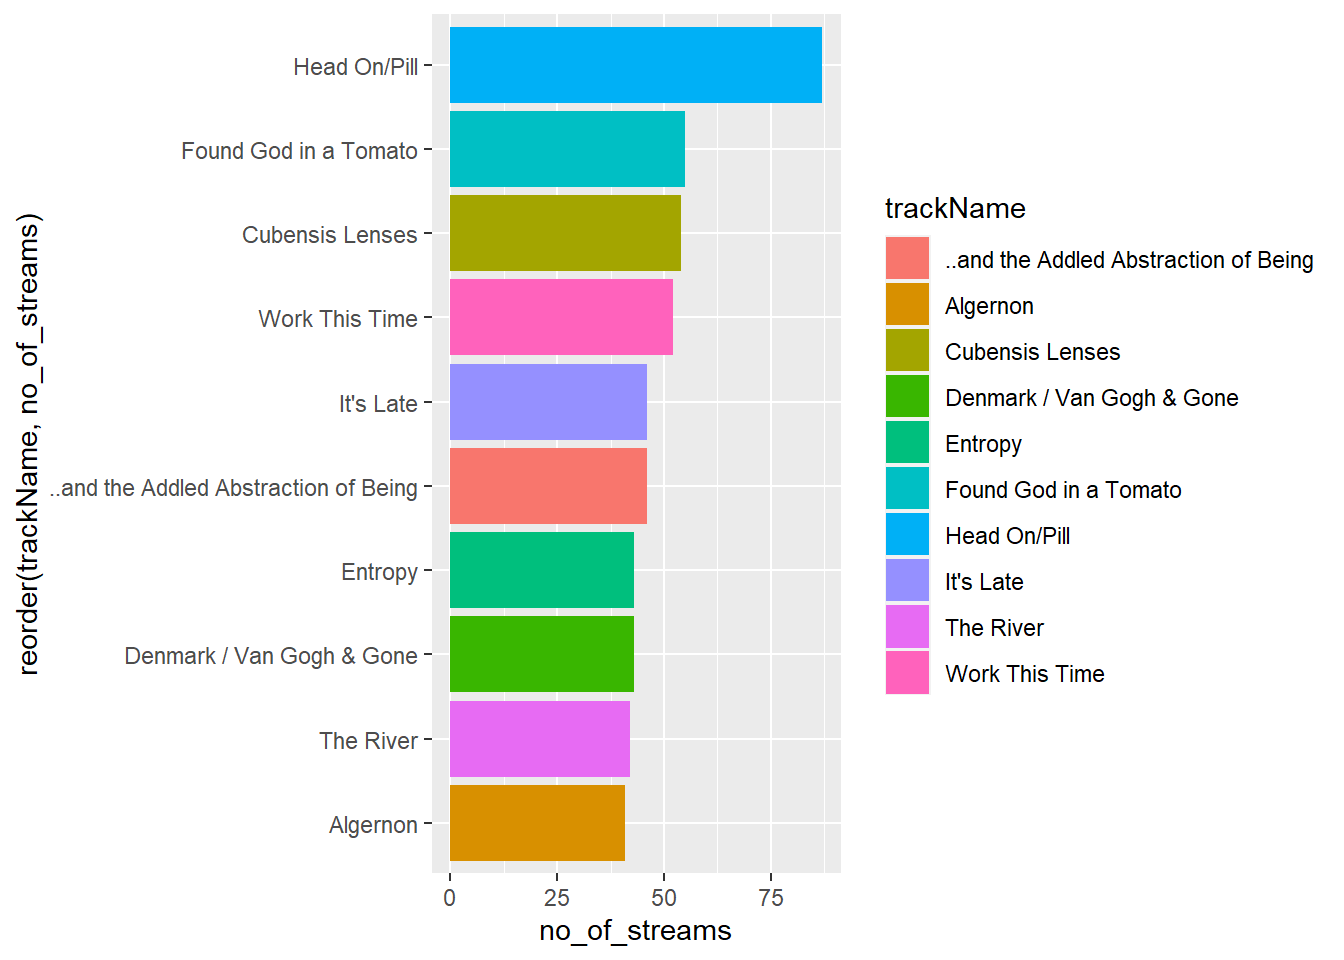
\includegraphics{spotify_eda_files/figure-latex/unnamed-chunk-3-1.pdf}

\hypertarget{by-minutes}{%
\subparagraph{By minutes}\label{by-minutes}}

\begin{Shaded}
\begin{Highlighting}[]
\NormalTok{songs }\OperatorTok\StringTok{ }\KeywordTok{ggplot}\NormalTok{(}\KeywordTok{aes}\NormalTok{(}\DataTypeTok{x=}\KeywordTok{reorder}\NormalTok{(trackName, total_minutes), }\DataTypeTok{y=}\NormalTok{total_minutes)) }\OperatorTok{+}\StringTok{ }
\StringTok{  }\KeywordTok{geom_bar}\NormalTok{(}\DataTypeTok{stat=}\StringTok{"identity"}\NormalTok{, }\KeywordTok{aes}\NormalTok{(}\DataTypeTok{fill=}\NormalTok{trackName)) }\OperatorTok{+}\StringTok{ }\KeywordTok{coord_flip}\NormalTok{()}
\end{Highlighting}
\end{Shaded}

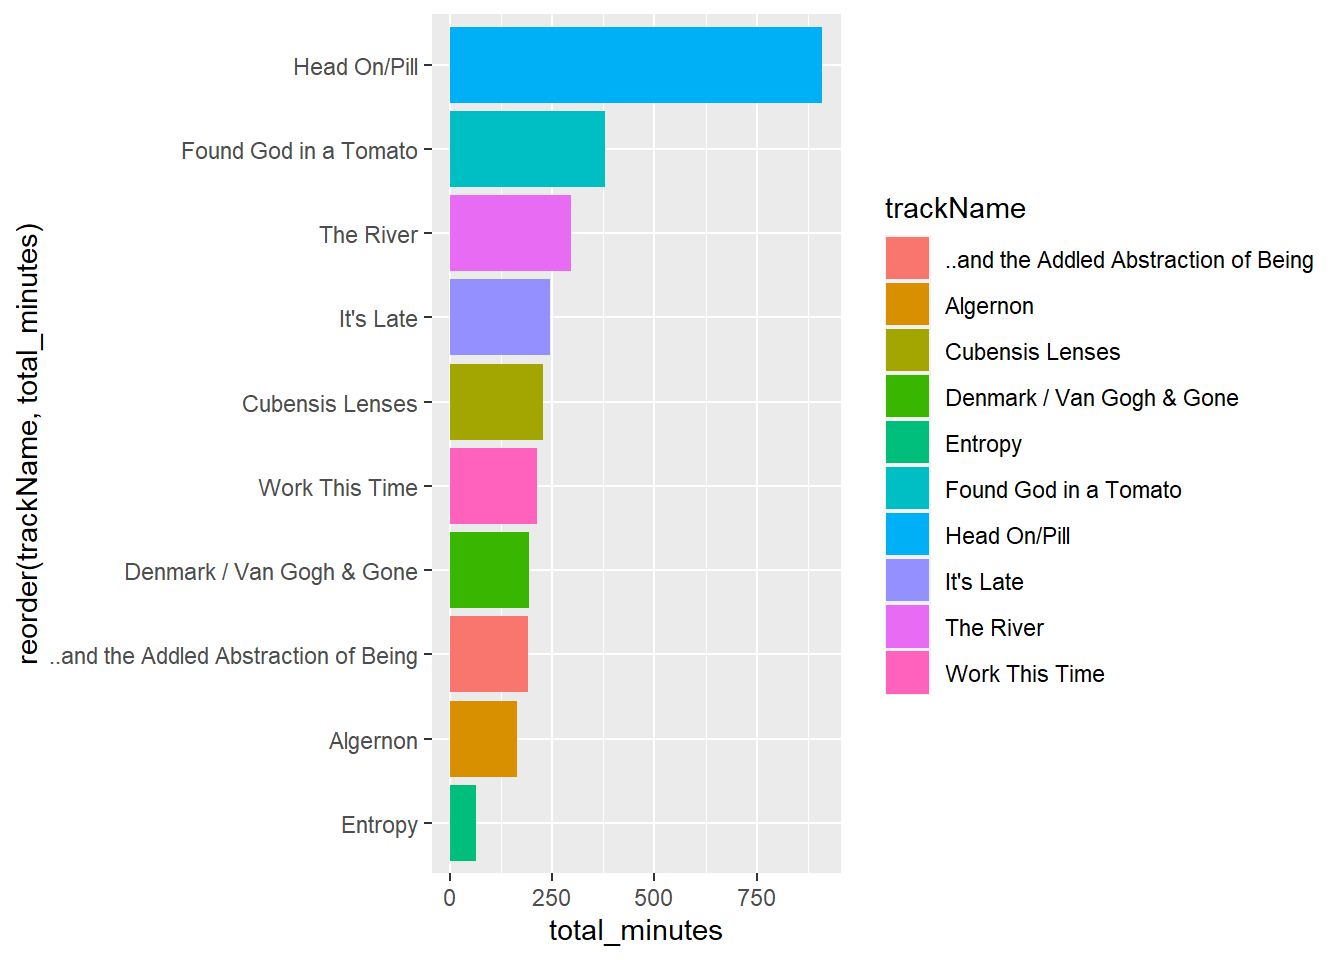
\includegraphics{spotify_eda_files/figure-latex/unnamed-chunk-4-1.pdf}

\hypertarget{longest-songs}{%
\paragraph{Longest songs}\label{longest-songs}}

\begin{Shaded}
\begin{Highlighting}[]
\NormalTok{spotify }\OperatorTok\StringTok{ }
\StringTok{  }\KeywordTok{filter}\NormalTok{(completed}\OperatorTok{==}\DecValTok{1}\NormalTok{) }\OperatorTok
\StringTok{  }\KeywordTok{distinct}\NormalTok{(artistName, trackName, duration_ms) }\OperatorTok
\StringTok{  }\KeywordTok{mutate}\NormalTok{(}\DataTypeTok{runtime_mins =}\NormalTok{ duration_ms}\OperatorTok{/}\DecValTok{60000}\NormalTok{) }\OperatorTok
\StringTok{  }\KeywordTok{arrange}\NormalTok{(}\KeywordTok{desc}\NormalTok{(runtime_mins)) }\OperatorTok\StringTok{ }\KeywordTok{head}\NormalTok{(}\DecValTok{10}\NormalTok{) }\OperatorTok
\StringTok{  }\KeywordTok{ggplot}\NormalTok{(}\KeywordTok{aes}\NormalTok{(}\DataTypeTok{x=}\KeywordTok{reorder}\NormalTok{(trackName, runtime_mins), }\DataTypeTok{y=}\NormalTok{runtime_mins)) }\OperatorTok{+}
\StringTok{  }\KeywordTok{geom_bar}\NormalTok{(}\DataTypeTok{stat=}\StringTok{"identity"}\NormalTok{, }\KeywordTok{aes}\NormalTok{(}\DataTypeTok{fill=}\NormalTok{trackName)) }\OperatorTok{+}\StringTok{ }\KeywordTok{coord_flip}\NormalTok{()}
\end{Highlighting}
\end{Shaded}

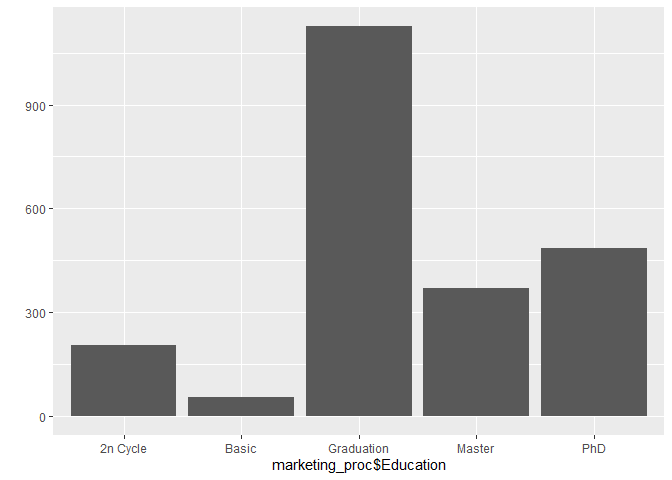
\includegraphics{spotify_eda_files/figure-latex/unnamed-chunk-5-1.pdf}

\hypertarget{artist-level-aggregates}{%
\subsection{Artist Level Aggregates}\label{artist-level-aggregates}}

\hypertarget{most-listened-artists-by-total-number-of-songs-played-distinct-albums-listened-to-total-duration-listened-to}{%
\paragraph{Most listened Artists by total number of songs played,
distinct albums listened to, total duration listened
to}\label{most-listened-artists-by-total-number-of-songs-played-distinct-albums-listened-to-total-duration-listened-to}}

\begin{Shaded}
\begin{Highlighting}[]
\NormalTok{artists <-}\StringTok{ }\NormalTok{spotify }\OperatorTok
\StringTok{  }\KeywordTok{group_by}\NormalTok{(artistName) }\OperatorTok
\StringTok{  }\KeywordTok{summarise}\NormalTok{(}\DataTypeTok{songs_played=}\KeywordTok{n}\NormalTok{(), }\DataTypeTok{distinct_songs=}\KeywordTok{n_distinct}\NormalTok{(trackName),}
            \DataTypeTok{distinct_albums=}\KeywordTok{n_distinct}\NormalTok{(albumName), }\DataTypeTok{total_duration_hours=}\KeywordTok{sum}\NormalTok{(msPlayed)}\OperatorTok{/}\DecValTok{3600000}\NormalTok{,}
            \DataTypeTok{completed_songs=}\KeywordTok{sum}\NormalTok{(completed)) }\OperatorTok
\StringTok{  }\KeywordTok{arrange}\NormalTok{(}\KeywordTok{desc}\NormalTok{(songs_played)) }\OperatorTok\StringTok{ }\KeywordTok{head}\NormalTok{(}\DecValTok{10}\NormalTok{)}
\NormalTok{artists}
\end{Highlighting}
\end{Shaded}

\begin{verbatim}
## # A tibble: 10 x 6
##    artistName songs_played distinct_songs distinct_albums total_duration_~
##    <chr>             <int>          <int>           <int>            <dbl>
##  1 King Gizz~          797             88              15            56.6 
##  2 Psychedel~          451             35               5            26.7 
##  3 Sufjan St~          257             39              10             9.16
##  4 A Beacon ~          184             11               1            10.1 
##  5 Kikagaku ~          147             18               5             9.77
##  6 Crumb               104             14               3             5.47
##  7 MGMT                 99             21               6             5.90
##  8 Mort Gars~           63             14               2             2.74
##  9 Radiohead            63             25               5             3.49
## 10 Feng Suave           54              6               5             3.00
## # ... with 1 more variable: completed_songs <dbl>
\end{verbatim}

\begin{Shaded}
\begin{Highlighting}[]
\NormalTok{artists }\OperatorTok\StringTok{ }\KeywordTok{ggplot}\NormalTok{(}\KeywordTok{aes}\NormalTok{(}\DataTypeTok{x=}\KeywordTok{reorder}\NormalTok{(artistName, songs_played), }\DataTypeTok{y=}\NormalTok{songs_played)) }\OperatorTok{+}\StringTok{ }
\StringTok{  }\KeywordTok{geom_bar}\NormalTok{(}\DataTypeTok{stat=}\StringTok{"identity"}\NormalTok{, }\KeywordTok{aes}\NormalTok{(}\DataTypeTok{fill=}\NormalTok{artistName)) }\OperatorTok{+}\StringTok{ }\KeywordTok{coord_flip}\NormalTok{()}
\end{Highlighting}
\end{Shaded}

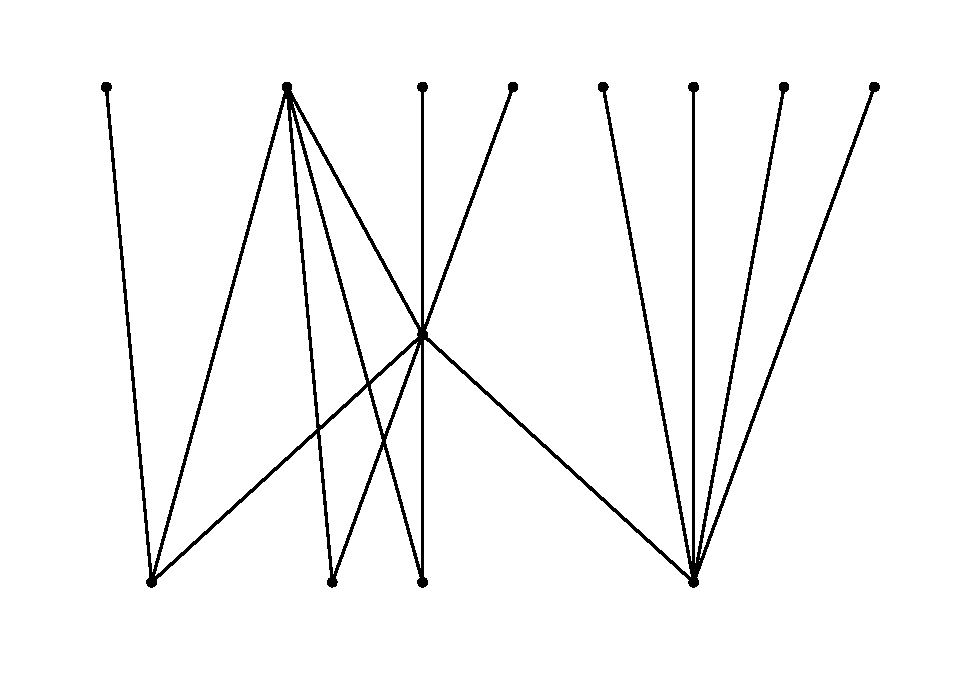
\includegraphics{spotify_eda_files/figure-latex/unnamed-chunk-7-1.pdf}

\begin{Shaded}
\begin{Highlighting}[]
\NormalTok{artists }\OperatorTok\StringTok{ }\KeywordTok{ggplot}\NormalTok{(}\KeywordTok{aes}\NormalTok{(}\DataTypeTok{x=}\NormalTok{artistName, }\DataTypeTok{y=}\NormalTok{songs_played)) }\OperatorTok{+}\StringTok{ }
\StringTok{  }\KeywordTok{geom_bar}\NormalTok{(}\DataTypeTok{stat=}\StringTok{"identity"}\NormalTok{, }\KeywordTok{aes}\NormalTok{(}\DataTypeTok{fill=}\NormalTok{artistName)) }\OperatorTok{+}\StringTok{ }\KeywordTok{coord_flip}\NormalTok{()}
\end{Highlighting}
\end{Shaded}

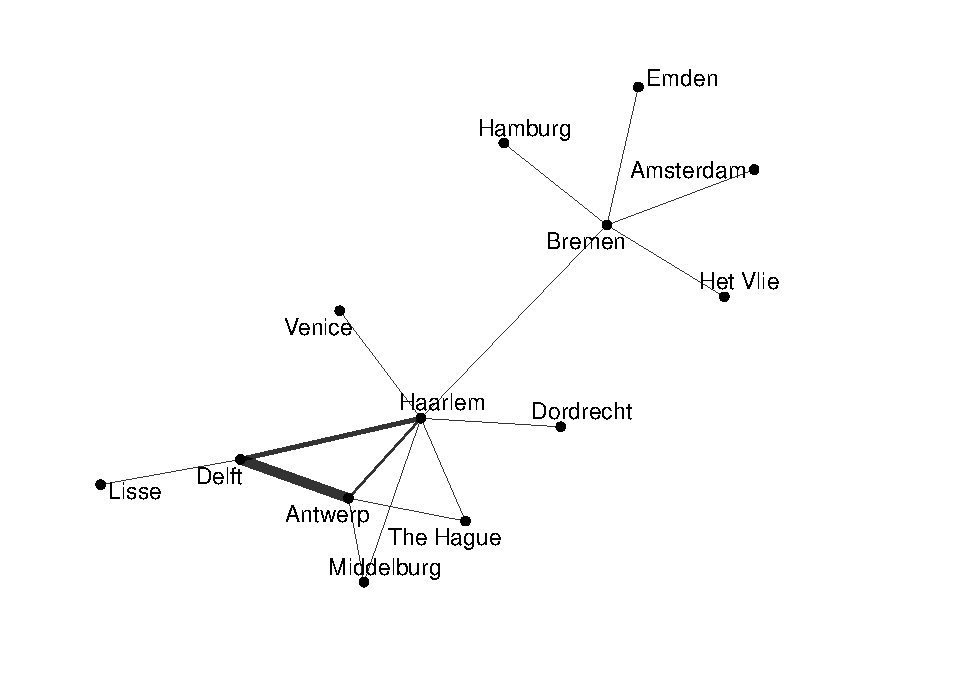
\includegraphics{spotify_eda_files/figure-latex/unnamed-chunk-8-1.pdf}


\end{document}
